\documentclass[a4paper]{article}
\usepackage[utf8]{inputenc} % Кодировка UTF-8
\usepackage[english,russian]{babel}
\usepackage[T2A]{fontenc} % Для кириллицы
\usepackage{graphicx} % Required for inserting images
\usepackage{listings}
\usepackage{xcolor}
\usepackage{tabularx}
\usepackage{booktabs}
\usepackage{caption}
\usepackage{amsmath}

\lstdefinestyle{mystyle}{
    backgroundcolor=\color{white},   % цвет фона
    commentstyle=\color{green},          % цвет комментариев
    keywordstyle=\color{blue},           % цвет ключевых слов
    numberstyle=\tiny\color{gray},       % стиль номера строк
    stringstyle=\color{red},             % цвет строк
    basicstyle=\ttfamily\footnotesize,   % основной стиль шрифта
    breakatwhitespace=false,              % перенос строк только по пробелам
    breaklines=true,                      % перенос длинных строк
    numbers=left,                        % номера строк слева
    numbersep=5pt,                       % расстояние между номером строки и кодом
    tabsize=2,                           % размер табуляции
}

\lstset{style=mystyle} % Применяем стиль


\begin{document}

\begin{titlepage}
    \centering
    {\Large МИНИСТЕРСТВО ОБРАЗОВАНИЯ И НАУКИ РОССИЙСКОЙ ФЕДЕРАЦИИ \\[1em]
    Федеральное государственное автономное образовательное учреждение  \\[1em]
    высшего образования \\[1em]
    \textbf{<<Национальный исследовательский \\ Нижегородский государственный университет \\ 
    им. Н.И. Лобачевского>> \\ (ННГУ) \\[1em]
    Институт информационных технологий, математики и механики}}
    
    \vspace{1cm}
    {\Huge \textbf{Отчет} \\[1em]
    Построение выпуклой оболочки - метод Джарвиса. MPI}
    
    \vspace{1cm}
    \raggedleft
    {\textbf{Группа: 3822Б1ПР2 \\ Автор: Владимирова Юлия\\лектор: Сысоев\\ Александр Владимирович\\ доцент, кандидат технических наук\\преподаватель: Оболенский Арсений\\ Андреевич\\преподаватель: Нестеров Александр\\ Юрьевич\\}}
        \vspace{2cm}
   \centering  {\textbf{26 декабря 2024 г.}}
\end{titlepage}

\section{Введение}
\hspace{1cm}{Данный документ является отчетом к лабораторной работе №3 по предмету <<Параллельное программирование>>}

\textbf{Задача звучит так:} на вход подается черно-белое изображение, содержащее в себе точки. Необходимо построить выпуклую оболочку для этих точек.



\section{Теоритическая часть}

\hspace{0.5cm} В моей задаче необходимо найти минимальную выпуклую оболочку. Выпуклой оболочкой называется кривая H без самопересечений, такая, что все точки множества лежат внутри этой кривой. Если кривая H является выпуклой (например, любая касательная к этой кривой не пересекает ее больше ни в одной точке), то соответствующая оболочка также называется выпуклой.

\textbf{Алгоритм Джарвиса}

Алгоритм Джарвиса является двухшаговым. Изначально необходимо взять точку, точно входящую в оболочку. В оболочку точно входит граничная точка, легче всего найти граничные точки по осям координат, то есть самую левую, правую, верхнюю, нижнюю. Принято и удобно брать самую нижнюю левую точку.

Через первую точку проводится горизонтальная прямая. Находим точку, составляющую с этой прямой минимальный угол (по часовой стрелке).

Теперь у нас есть две точки, через них необходимо провести прямую и найти точку, которая составляет минимальный угол уже с этой прямой.


\section{Преобразование и создание алгоритма}
\hspace{1cm}Для того чтобы вычислить угол, я решила использовать \textbf{формулу для нахождения угла между векторами \(\mathbf{\vec{a}}\) и \(\mathbf{\vec{b}}\)}:

\[
\cos(\theta) = \frac{\mathbf{\vec{a}} \cdot \mathbf{\vec{b}}}{\|\mathbf{\vec{a}}\| \|\mathbf{\vec{b}}\|}
\]
\\
Первую точку назовем \textbf{A}, вторую точку \textbf{B}, а искомую \textbf{C}\\
Т.к. мы теперь используем вектор, а не прямую, правильным будет поменять измеряемый угол, ведь до этого у нас вычислялся угол с прямой, которая точно будет дальше точки C, а сейчас у нас вектор, который имеет длину, поэтому угол $\alpha$ \text{меняем на} $\beta$ . То есть мы применяем правило смежных углов, они пропроциональные и их значения в сумме дают 180$^\circ$


\begin{figure}[h] % "h" означает, что изображение будет вставлено "здесь"
    \centering % Центрирование изображения
    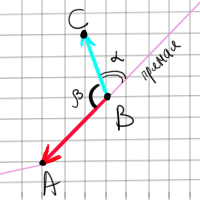
\includegraphics[width=0.2\textwidth]{image1.png} % Замените путь на путь к вашему изображению
    \caption{} % Подпись к изображению
    \label{fig:example} % Метка для ссылки на изображение
\end{figure}

Учитывая то, что нам необходимо было найти наименьший угол  $\alpha$ , и то, что чем больше угол $\beta$ , тем меньше угол  $\alpha$ , то необходимо найти наибольший угол $\beta$ .  Чем больше угол, тем меньше его косинус. Это можно рассмотреть на единичной окружности, косинус берется по оси x.

\begin{figure}[h] % "h" означает, что изображение будет вставлено "здесь"
    \centering % Центрирование изображения
    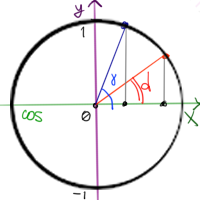
\includegraphics[width=0.45\textwidth]{image2.png} % Замените путь на путь к вашему изображению
    \caption{} % Подпись к изображению
    \label{fig:example} % Метка для ссылки на изображение
\end{figure}

В итоге мы пришли к тому, что необходимо найти наименьший косинус угла.
\\
\textbf{Алгоритм}\\
Алгоритм состоит из двух частей:\\
\textit{Нахождение первой точки}
Т.к. изображение двумерное - соответсвенно это вектор, если мы построчно рассматриваем кратинку, то необходимо найти последнюю точку в векторе, а потом перебирать точки в обратном порядке, пока следующая точка не уйдет на более высокую координату y. В данном случае более высокая координата у - это ее меньшее значение, т.к. изображение рассматриваем с левого верхнего угла. 


\begin{figure}[h] % "h" означает, что изображение будет вставлено "здесь"
    \centering % Центрирование изображения
    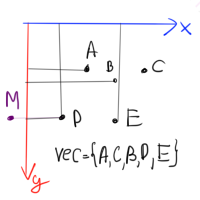
\includegraphics[width=0.45\textwidth]{image3.png} % Замените путь на путь к вашему изображению
    \caption{} % Подпись к изображению
    \label{fig:example} % Метка для ссылки на изображение
\end{figure}
 После этого необходимо сохранить найденную точку, ведь мы собираемся к ней вернуться.
 Необходимо провести горизонтальный вектор, чтобы точно не попасть ни в какую точку, мы возьмем мнимую точку \textbf{M}, которая имеет отрицательный х. Проведем вектор между этими двумя точками.
 \textit{Нахождение точки C}
 Мы будем перебирать все точки в поисках минимального косинуса. После того, как мы нашли точку C с минимальным косинусом, мы убираем предыдущую точку А и точки B, С из рассматриваемых. Теперь A:=B, B:=C. Если B не равен самой первой точке в оболочке - запускаем нахождение минимальной точки С еще раз.\\
 
\textbf{Код}
\begin{lstlisting}[language=C++, caption=Первая часть алгоритма:, label=lst:example]
Point* A = &input_[input_.size() - 1];
for (size_t i = input_.size() - 1; i >= 0; i--) { 
    if (A->y != input_[i].y) break;
    A = &input_[i];
}
\end{lstlisting}

\begin{lstlisting}[language=C++, caption=Вторая часть алгоритма:, label=lst:example]
first = A;
Point tmp = vladimirova_j_jarvis_method_seq::Point(-1, A->y);
Point* B = A;
A = &tmp;
res_ = std::vector<int>();
do {
  size_t i = FindMinAngle(A, B, input_);
  if (A != first) {
    A->x = -1;
    A->y = -1;
  }
  A = B;
  res_.push_back(A->y);
  res_.push_back(A->x);
  B = &input_[i];

} while (B != first);
\end{lstlisting}

\begin{lstlisting}[language=C++, caption=Формула нахождения минимального угла:, label=lst:example]
size_t min_angle_point = vec.size() + 1;
double min_angle = 550;
int reg_x = A->x - (B->x);
int reg_y = -(A->y - B->y); 
for (size_t i = 0; i < vec.size(); i++) {
  Point* C = &vec[i];
  if (C->x < 0) continue;
  if ((A->x == C->x) && (A->y == C->y)) continue;
  if ((B->x == C->x) && (B->y == C->y)) continue;
  int tmp_x = (C->x - B->x);
  int tmp_y = -(C->y - B->y);
  if (reg_x * tmp_y - reg_y * tmp_x <= 0) {
    double BA_length = sqrt(reg_x * reg_x + reg_y * reg_y);
    double BC_length = sqrt(tmp_x * tmp_x + tmp_y * tmp_y);
    double length = BA_length * BC_length;
    double angle = tmp_x * reg_x + tmp_y * reg_y;
    if (length == 0)
      angle = 0;
    else
      angle = angle / (length);
    if (angle < min_angle) {
      min_angle = angle;
      min_angle_point = i;
    }
  }
}

return min_angle_point;
}
\end{lstlisting}
Тут все уже просмотренные точки получают координату -1, мне показалось это лучше чем удалять их из вектора. 



\section{Распараллеливание работы}
\hspace{1cm} Если у нас есть несколько процессов, то можно разделить перебор возможных точек C. Необходимо только разделить работу, все остальное остается прежним.
Я взяла такой способ распараллеливания: поделила точки между процессами, каждый процесс считает косинус лишь для своих точек, сам находит минимум и возвращает свой "лучший" результат. 


\begin{figure}[h] % "h" означает, что изображение будет вставлено "здесь"
    \centering % Центрирование изображения
    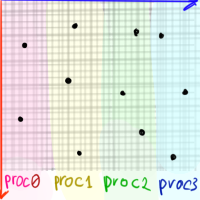
\includegraphics[width=0.45\textwidth]{image4.png} % Замените путь на путь к вашему изображению
    \caption{} % Подпись к изображению
    \label{fig:example} % Метка для ссылки на изображение
\end{figure}

Длину вектора \(\vec{AB}\)\ вычисляет только 0-ой процесс, и уже передает длину вместе с координатами точки B.
Если процесс понимает, что переданная точка B находится в его зоне, то он удаляет эту точку из рассматриваемых точек (кроме самой первой итерации, чтоб случайно не удалить первую точку в оболочке, ведь нам надо к ней вернуться).
Процесс 0 собирает все данные от процессов и находит наименьший результат из лучших, меняет точки A, B и С и начинает новую итерацию.
В случае если у процесса закончились точки, он ничего не считает, а просто отправляет "невозможно плохой вариант", то есть косинус угла >1. 
Если процесс 0 понял, что оболочка построена (что мы пришли к изначальной точке), то он оповещает об этом все процессы и завершается.\\\\

\textbf{Код}
\begin{lstlisting}[language=C++, caption=Распрараллеливание процесс 0:, label=lst:example]
 if (rank == 0) {
   B = Point(input_[input_.size() - 2], input_[input_.size() - 1]);
   Point A = Point(-1, -1);
   int j = input_.size() - 3;
   while (input_[j] == B.y) {
     B.x = input_[j - 1];
     j -= 2;
   }
   Point first = B;

   reg_x = -1;
   reg_y = 0;

   std::vector<int> send_data = {reg_x, reg_y, B.x, B.y, active};
   std::vector<double> send0_data(3);
   do {
     double min_angle = 1000;
     send_data = {reg_x, reg_y, B.x, B.y, 1};
     for (int i = 1; i < world.size(); i++) world.send(i, 0, send_data.data(), 5);
    
     std::vector<double> ans = getMinAngleMPI(reg_x, reg_y, B, local_input_, f);
     C = local_input_[(size_t)ans[0]];
     min_angle = ans[1];
     sz = (size_t)ans[2];
     for (int i = 1; i < world.size(); i++) {
       world.recv(i, 0, send0_data.data(), 3);
       if (send0_data[0] < min_angle) {
         C.x = (int)send0_data[1];
         C.y = (int)send0_data[2];
       }
     }

     res_.push_back(B.y);
     res_.push_back(B.x);
     A = B;
     B = C;
     reg_x = A.x - (B.x);
     reg_y = -(A.y - B.y); 
     f = true;
   } while (first != B);
   send_data[4] = 0;
   for (int i = 1; i < world.size(); i++) world.send(i, 0, send_data.data(), 5);
 }

\end{lstlisting}


\begin{lstlisting}[language=C++, caption=Распрараллеливание Процесс 0:, label=lst:example]
 if (rank == 0) {
   B = Point(input_[input_.size() - 2], input_[input_.size() - 1]);
   Point A = Point(-1, -1);
   int j = input_.size() - 3;
   while (input_[j] == B.y) {
     B.x = input_[j - 1];
     j -= 2;
   }
   Point first = B;

   reg_x = -1;
   reg_y = 0;

   std::vector<int> send_data = {reg_x, reg_y, B.x, B.y, active};
   std::vector<double> send0_data(3);
   do {
     double min_angle = 1000;
     send_data = {reg_x, reg_y, B.x, B.y, 1};
     for (int i = 1; i < world.size(); i++) world.send(i, 0, send_data.data(), 5);
     std::vector<double> ans = getMinAngleMPI(reg_x, reg_y, B, local_input_, f);
     C = local_input_[(size_t)ans[0]];
     min_angle = ans[1];
     sz = (size_t)ans[2];
     for (int i = 1; i < world.size(); i++) {
       world.recv(i, 0, send0_data.data(), 3);
       if (send0_data[0] < min_angle) {
         C.x = (int)send0_data[1];
         C.y = (int)send0_data[2];
       }
     }

     res_.push_back(B.y);
     res_.push_back(B.x);
     A = B;
     B = C;
     reg_x = A.x - (B.x);
     reg_y = -(A.y - B.y); 
     f = true;
   } while (first != B);
   send_data[4] = 0;
   for (int i = 1; i < world.size(); i++) world.send(i, 0, send_data.data(), 5);
 }

\end{lstlisting}


\begin{lstlisting}[language=C++, caption=Распрараллеливание Процесс не 0:, label=lst:example]
 
  if (rank != 0) {
    std::vector<int> send_data(5);
    std::vector<double> send0_data(3);
    while (active == 1) {
      world.recv(0, 0, send_data.data(), 5);
      active = send_data[4];
      if (active != 1) return true;
      if (sz <= 0) {
        send0_data = {10000, -1, -1};
        world.send(0, 0, send0_data.data(), 3);
        continue;
      }
      B.x = send_data[2];
      B.y = send_data[3];
      double min_angle = 5000;
      std::vector<double> ans = getMinAngleMPI(send_data[0], send_data[1], B, local_input_, f);
      f = true;
      size_t itr = ans[0];
      C = local_input_[itr];
      min_angle = ans[1];
      sz = (size_t)ans[2];
      send0_data = {min_angle, (double)C.x, (double)C.y};
      world.send(0, 0, send0_data.data(), 3);
    }
  }
\end{lstlisting}


\section{Валидация}
\hspace{1cm}{
Чтобы построить оболочку есть несколько условий, а именно: точек должно быть больше двух, точки не должны стоять на одной прямой.
}

\section{Препроцессинг}
\hspace{1cm}{В препроцессинге я прохожусь по картинке-массиву, записываю только координаты x и y всех найденных точек, точками считаю все, что не белое, то есть имеет значение отличное от 255.}


\section{Работа}
\hspace{1cm}{Работа seq версии заключается в применении алгоритма, описанного выше. Работа mpi версии заключается в изначальном разделении работы (пункт распараллеливания работы), а после в каждом процессе применении алгоритма, описанного выше.}
\section{Постпроцессинг}
\hspace{1cm}{В постпроцессинге записываются точки, через которые проведена оболочка в соответственном порядке, в данном случае порядок необходимо сохранить, иначе оболочка будет совершенно другой. Также я записываю длину вывода.}

\section{Результат}
\hspace{1cm} Результат вышел таким (его нет в git, из-за ограничения по времени менее 1s)\\
\begin{table}[h]
    \centering
    \caption{Результаты теста для метода pipeline}
    \begin{tabular}{@{}ll@{}}
        \toprule
        \textbf{Метод seq} & \textbf{Метод mpi} \\
        \midrule
        1) 1,621302200 & 1) 0,836826 \\
        2) 1,1716390   & 2) 0,889073900 \\
        3) 1,1539773   & 3) 0,9007 \\
        \bottomrule
    \end{tabular}
\end{table}
\begin{table}[h]
    \centering
    \caption{Результаты теста}
    \begin{tabular}{@{}ll@{}} 
        \toprule
        \textbf{Метод seq} & \textbf{Метод mpi} \\
        \midrule
        1) 39,1089 & 1) 17,5670 \\
        2) 30,7824 & 2) 17,4288 \\
        3) 29,5636 & 3) 19,7248 \\
        \bottomrule
    \end{tabular}
\end{table}

\section{Вывод}
\hspace{1cm}{Существенное увеличение эффективности mpi версии видно с увеличением кол-ва данных. Я считаю, что я молодец и поставленная цель выполнена.}
\section{Литература}
\hspace{1cm} https://habr.com/ru/articles/144921/
https://www.youtube.com/watch?v=B2AJoQSZf4M
\section{Приложение}
Код 
\begin{lstlisting}[language=C++, caption=КОД:, label=lst:example]
#include "mpi/vladimirova_j_jarvis_method/include/ops_mpi.hpp"

#include <cmath>
#include <string>
#include <thread>
#include <vector>

using namespace std::chrono_literals;
using namespace vladimirova_j_jarvis_method_mpi;

namespace vladimirova_j_jarvis_method_mpi {
double getAngle(int reg_x, int reg_y, Point B, Point C) {
  if (C.x < 0) return 1000;
  if ((B.x == C.x) && (B.y == C.y)) return 1000;
  int tmp_x = (C.x - B.x);
  int tmp_y = -(C.y - B.y);
  if (reg_x * tmp_y - reg_y * tmp_x > 0) return 1000;
  double BA_length = sqrt(reg_x * reg_x + reg_y * reg_y);
  double BC_length = sqrt(tmp_x * tmp_x + tmp_y * tmp_y);
  double length = BA_length * BC_length;
  double angle = tmp_x * reg_x + tmp_y * reg_y;
  if (length == 0)
    angle = 0;
  else
    angle = angle / (length);
  return angle;
}
std::vector<double> getMinAngleMPI(int reg_x, int reg_y, Point B, std::vector<Point>& vec, bool f) {
  size_t min_angle_point = vec.size() + 1;
  double min_angle = 550;
  size_t sz = 0;
  for (size_t i = 0; i < vec.size(); i++) {
    if (f && (vec[i] == B)) {
      vec[i].x = -1;
      vec[i].y = -1;
      continue;
    }
    if (vec[i].x < 0) continue;
    double angle = getAngle(reg_x, reg_y, B, vec[i]);
    if (angle < min_angle) {
      min_angle = angle;
      min_angle_point = i;
    }
    sz++;
  }
  return {(double)min_angle_point, min_angle, (double)sz};
}

size_t FindMinAngle(Point* A, Point* B, std::vector<Point> vec) {
  size_t min_angle_point = vec.size() + 1;
  double min_angle = 550;
  int reg_x = A->x - (B->x);
  int reg_y = -(A->y - B->y); 
  for (size_t i = 0; i < vec.size(); i++) {
    Point* C = &vec[i];
    if (C->x < 0) continue;
    if ((A->x == C->x) && (A->y == C->y)) continue;
    if ((B->x == C->x) && (B->y == C->y)) continue;
    int tmp_x = (C->x - B->x);
    int tmp_y = -(C->y - B->y);
    if (reg_x * tmp_y - reg_y * tmp_x <= 0) {
      double BA_length = sqrt(reg_x * reg_x + reg_y * reg_y);
      double BC_length = sqrt(tmp_x * tmp_x + tmp_y * tmp_y);
      double length = BA_length * BC_length;
      double angle = tmp_x * reg_x + tmp_y * reg_y;
      if (length == 0)
        angle = 0;
      else
        angle = angle / (length);
      if (angle < min_angle) {
        min_angle = angle;
        min_angle_point = i;
      }
    }
  }

  return min_angle_point;
}
}  // namespace vladimirova_j_jarvis_method_mpi

bool vladimirova_j_jarvis_method_mpi::TestMPITaskSequential::pre_processing() {
  internal_order_test();
  input_ = std::vector<Point>();
  col = (size_t)taskData->inputs_count[1];
  row = (size_t)taskData->inputs_count[0];
  auto* tmp_ptr = reinterpret_cast<int*>(taskData->inputs[0]);
  for (size_t i = 0; i < col * row; i++) {
    if (tmp_ptr[i] != 255) {
      input_.emplace_back((int)(i % col), (int)(i / col));
    }
  }
  return true;
}

bool vladimirova_j_jarvis_method_mpi::TestMPITaskSequential::validation() {
  internal_order_test();
  // Check count elements of output
  size_t row_i = taskData->inputs_count[0];
  size_t col_i = taskData->inputs_count[1];
  if (row_i <= 1 || col_i <= 1 || taskData->outputs_count[0] <= 0) return false;
  auto* tmp_ptr = reinterpret_cast<int*>(taskData->inputs[0]);
  size_t c = 0;
  int one_row = -1;
  int one_col = -1;
  for (size_t i = 0; i < row_i * col_i; i++) {
    if (tmp_ptr[i] != 255) {
      c++;
      if (one_row == -1)
        one_row = i / row_i;
      else if ((one_row != -2) && (one_row != (int)(i / row_i)))
        one_row = -2;

      if (one_col == -1)
        one_col = i % row_i;
      else if ((one_col != -2) && (one_col != (int)(i % row_i)))
        one_col = -2;
    }
    if ((one_row == -2) && (one_col == -2) && (c > 2)) return true;
  }
  return ((c > 2) && (one_row == -2) && (one_col == -2));
}

bool vladimirova_j_jarvis_method_mpi::TestMPITaskSequential::run() {
  internal_order_test();
  Point* A = &input_[input_.size() - 1];
  for (size_t i = input_.size() - 1; i >= 0; i--) {  
    if (A->y != input_[i].y) break;
    A = &input_[i];
  }
  Point* first = A;
  Point tmp = Point(-1, A->y);

  Point* B = A;
  A = &tmp;
  res_ = std::vector<int>();
  do {
    size_t i = FindMinAngle(A, B, input_);
    if (A != first) {
      A->x = -1;
      A->y = -1;
    }
    A = B;
    res_.push_back(A->y);
    res_.push_back(A->x);
    B = &input_[i];

  } while (B != first);

  return true;
}

bool vladimirova_j_jarvis_method_mpi::TestMPITaskSequential::post_processing() {
  internal_order_test();
  taskData->outputs_count[0] = res_.size();
  auto* output_data = reinterpret_cast<int*>(taskData->outputs[0]);
  std::copy(res_.begin(), res_.end(), output_data);
  return true;
}

bool vladimirova_j_jarvis_method_mpi::TestMPITaskParallel::pre_processing() {
  internal_order_test();
  if (world.rank() == 0) {
    col = (size_t)taskData->inputs_count[1];
    row = (size_t)taskData->inputs_count[0];
  }
  broadcast(world, col, 0);
  broadcast(world, row, 0);
  if (world.rank() != 0) return true;

  input_ = std::vector<int>();

  auto* tmp_ptr = reinterpret_cast<int*>(taskData->inputs[0]);
  for (size_t i = 0; i < col * row; i++) {
    if (tmp_ptr[i] != 255) {
      input_.push_back((int)(i % col));
      input_.push_back((int)(i / col));
    }
  }
  res_.clear();
  return true;
}

bool vladimirova_j_jarvis_method_mpi::TestMPITaskParallel::validation() {
  internal_order_test();
  if (world.rank() == 0) {
    size_t row_i = taskData->inputs_count[0];
    size_t col_i = taskData->inputs_count[1];
    if (row_i <= 1 || col_i <= 1 || taskData->outputs_count[0] <= 0) return false;
    auto* tmp_ptr = reinterpret_cast<int*>(taskData->inputs[0]);
    size_t c = 0;
    int one_row = -1;
    int one_col = -1;
    for (size_t i = 0; i < row_i * col_i; i++) {
      if (tmp_ptr[i] != 255) {
        c++;
        if (one_row == -1)
          one_row = i / row_i;
        else if ((one_row != -2) && (one_row != (int)(i / row_i)))
          one_row = -2;

        if (one_col == -1)
          one_col = i % row_i;
        else if ((one_col != -2) && (one_col != (int)(i % row_i)))
          one_col = -2;
      }
      if ((one_row == -2) && (one_col == -2) && (c > 2)) return true;
    }
    std::cout << "SOME" << std::endl;
    return ((c > 2) && (one_row == -2) && (one_col == -2));
  }
  return true;
}

bool vladimirova_j_jarvis_method_mpi::TestMPITaskParallel::run() {
  internal_order_test();

  int rank = world.rank();
  int delta = ((input_.size() / 2) / world.size()) * 2;
  int ost_point = (input_.size() - delta * world.size()) / 2;
  broadcast(world, delta, 0);
  broadcast(world, ost_point, 0);
  if (rank == 0) {
    if (world.size() != 1) {
      for (int i = 1; i < ost_point; i++) {
        world.send(i, 0, input_.data() + i * (delta) + i * 2, delta + 2);
      }
      for (int i = ost_point + (int)(ost_point == 0); i < world.size(); i++) {
        int sdvig = ost_point * 2;
        world.send(i, 0, input_.data() + i * (delta) + sdvig, delta);
      }
      if (ost_point > 0) delta += 2;
    }
  } else {
    delta += 2 * (int)(rank < ost_point);
    input_ = std::vector<int>(delta);
    world.recv(0, 0, input_.data(), delta);
  }

  local_input_ = std::vector<Point>(delta / 2);

  for (int i = 0; i < delta; i += 2) {
    local_input_[i / 2] = (Point(input_[i], input_[i + 1]));
  }

  Point B = Point(-1, -1);
  Point C = Point(-1, -1);
  int reg_x;
  int reg_y;
  int active = 1;
  size_t sz = local_input_.size();
  bool f = false;
  if (rank == 0) {
    B = Point(input_[input_.size() - 2], input_[input_.size() - 1]);
    Point A = Point(-1, -1);
    int j = input_.size() - 3;
    while (input_[j] == B.y) {
      B.x = input_[j - 1];
      j -= 2;
    }
    Point first = B;

    reg_x = -1;
    reg_y = 0;
    std::vector<int> send_data = {reg_x, reg_y, B.x, B.y, active};
    std::vector<double> send0_data(3);
    do {
      double min_angle = 1000;
      send_data = {reg_x, reg_y, B.x, B.y, 1};
      for (int i = 1; i < world.size(); i++) world.send(i, 0, send_data.data(), 5);
      std::vector<double> ans = getMinAngleMPI(reg_x, reg_y, B, local_input_, f);
      C = local_input_[(size_t)ans[0]];
      min_angle = ans[1];
      sz = (size_t)ans[2];
      for (int i = 1; i < world.size(); i++) {
        world.recv(i, 0, send0_data.data(), 3);
        if (send0_data[0] < min_angle) {
          C.x = (int)send0_data[1];
          C.y = (int)send0_data[2];
        }
      }

      res_.push_back(B.y);
      res_.push_back(B.x);
      A = B;
      B = C;
      reg_x = A.x - (B.x);
      reg_y = -(A.y - B.y); 
      f = true;
    } while (first != B);
    send_data[4] = 0;
    for (int i = 1; i < world.size(); i++) world.send(i, 0, send_data.data(), 5);
  }

  if (rank != 0) {
    std::vector<int> send_data(5);
    std::vector<double> send0_data(3);
    while (active == 1) {
      world.recv(0, 0, send_data.data(), 5);
      active = send_data[4];
      if (active != 1) return true;
      if (sz <= 0) {
        send0_data = {10000, -1, -1};
        world.send(0, 0, send0_data.data(), 3);
        continue;
      }
      B.x = send_data[2];
      B.y = send_data[3];
      double min_angle = 5000;
      std::vector<double> ans = getMinAngleMPI(send_data[0], send_data[1], B, local_input_, f);
      f = true;
      size_t itr = ans[0];
      C = local_input_[itr];
      min_angle = ans[1];
      sz = (size_t)ans[2];
      send0_data = {min_angle, (double)C.x, (double)C.y};
      world.send(0, 0, send0_data.data(), 3);
    }
  }
  return true;
}

bool vladimirova_j_jarvis_method_mpi::TestMPITaskParallel::post_processing() {
  internal_order_test();
  if (world.rank() == 0) {
    taskData->outputs_count[0] = res_.size();
    auto* output_data = reinterpret_cast<int*>(taskData->outputs[0]);
    std::copy(res_.begin(), res_.end(), output_data);
    res_.clear();
    return true;
  }
  return true;
}

\end{lstlisting}
\end{document}
